\chapter{Platform}

The platform utilized on this project is the Nao humanoid experimental robotic platform by Aldebaran Robotics. It is a 25 degree-of-freedom humanoid mobile manipulator with two HD cameras, two ultrasonic distance sensors, four microphones, one three-axis accelerometer, two one-axis gyroscopes, and four force sensors in each foot. The platform is programmed using a framework called NAOqi allowing development using various languages including C++ and Python. 

\begin{figure}[h]
	\centering
	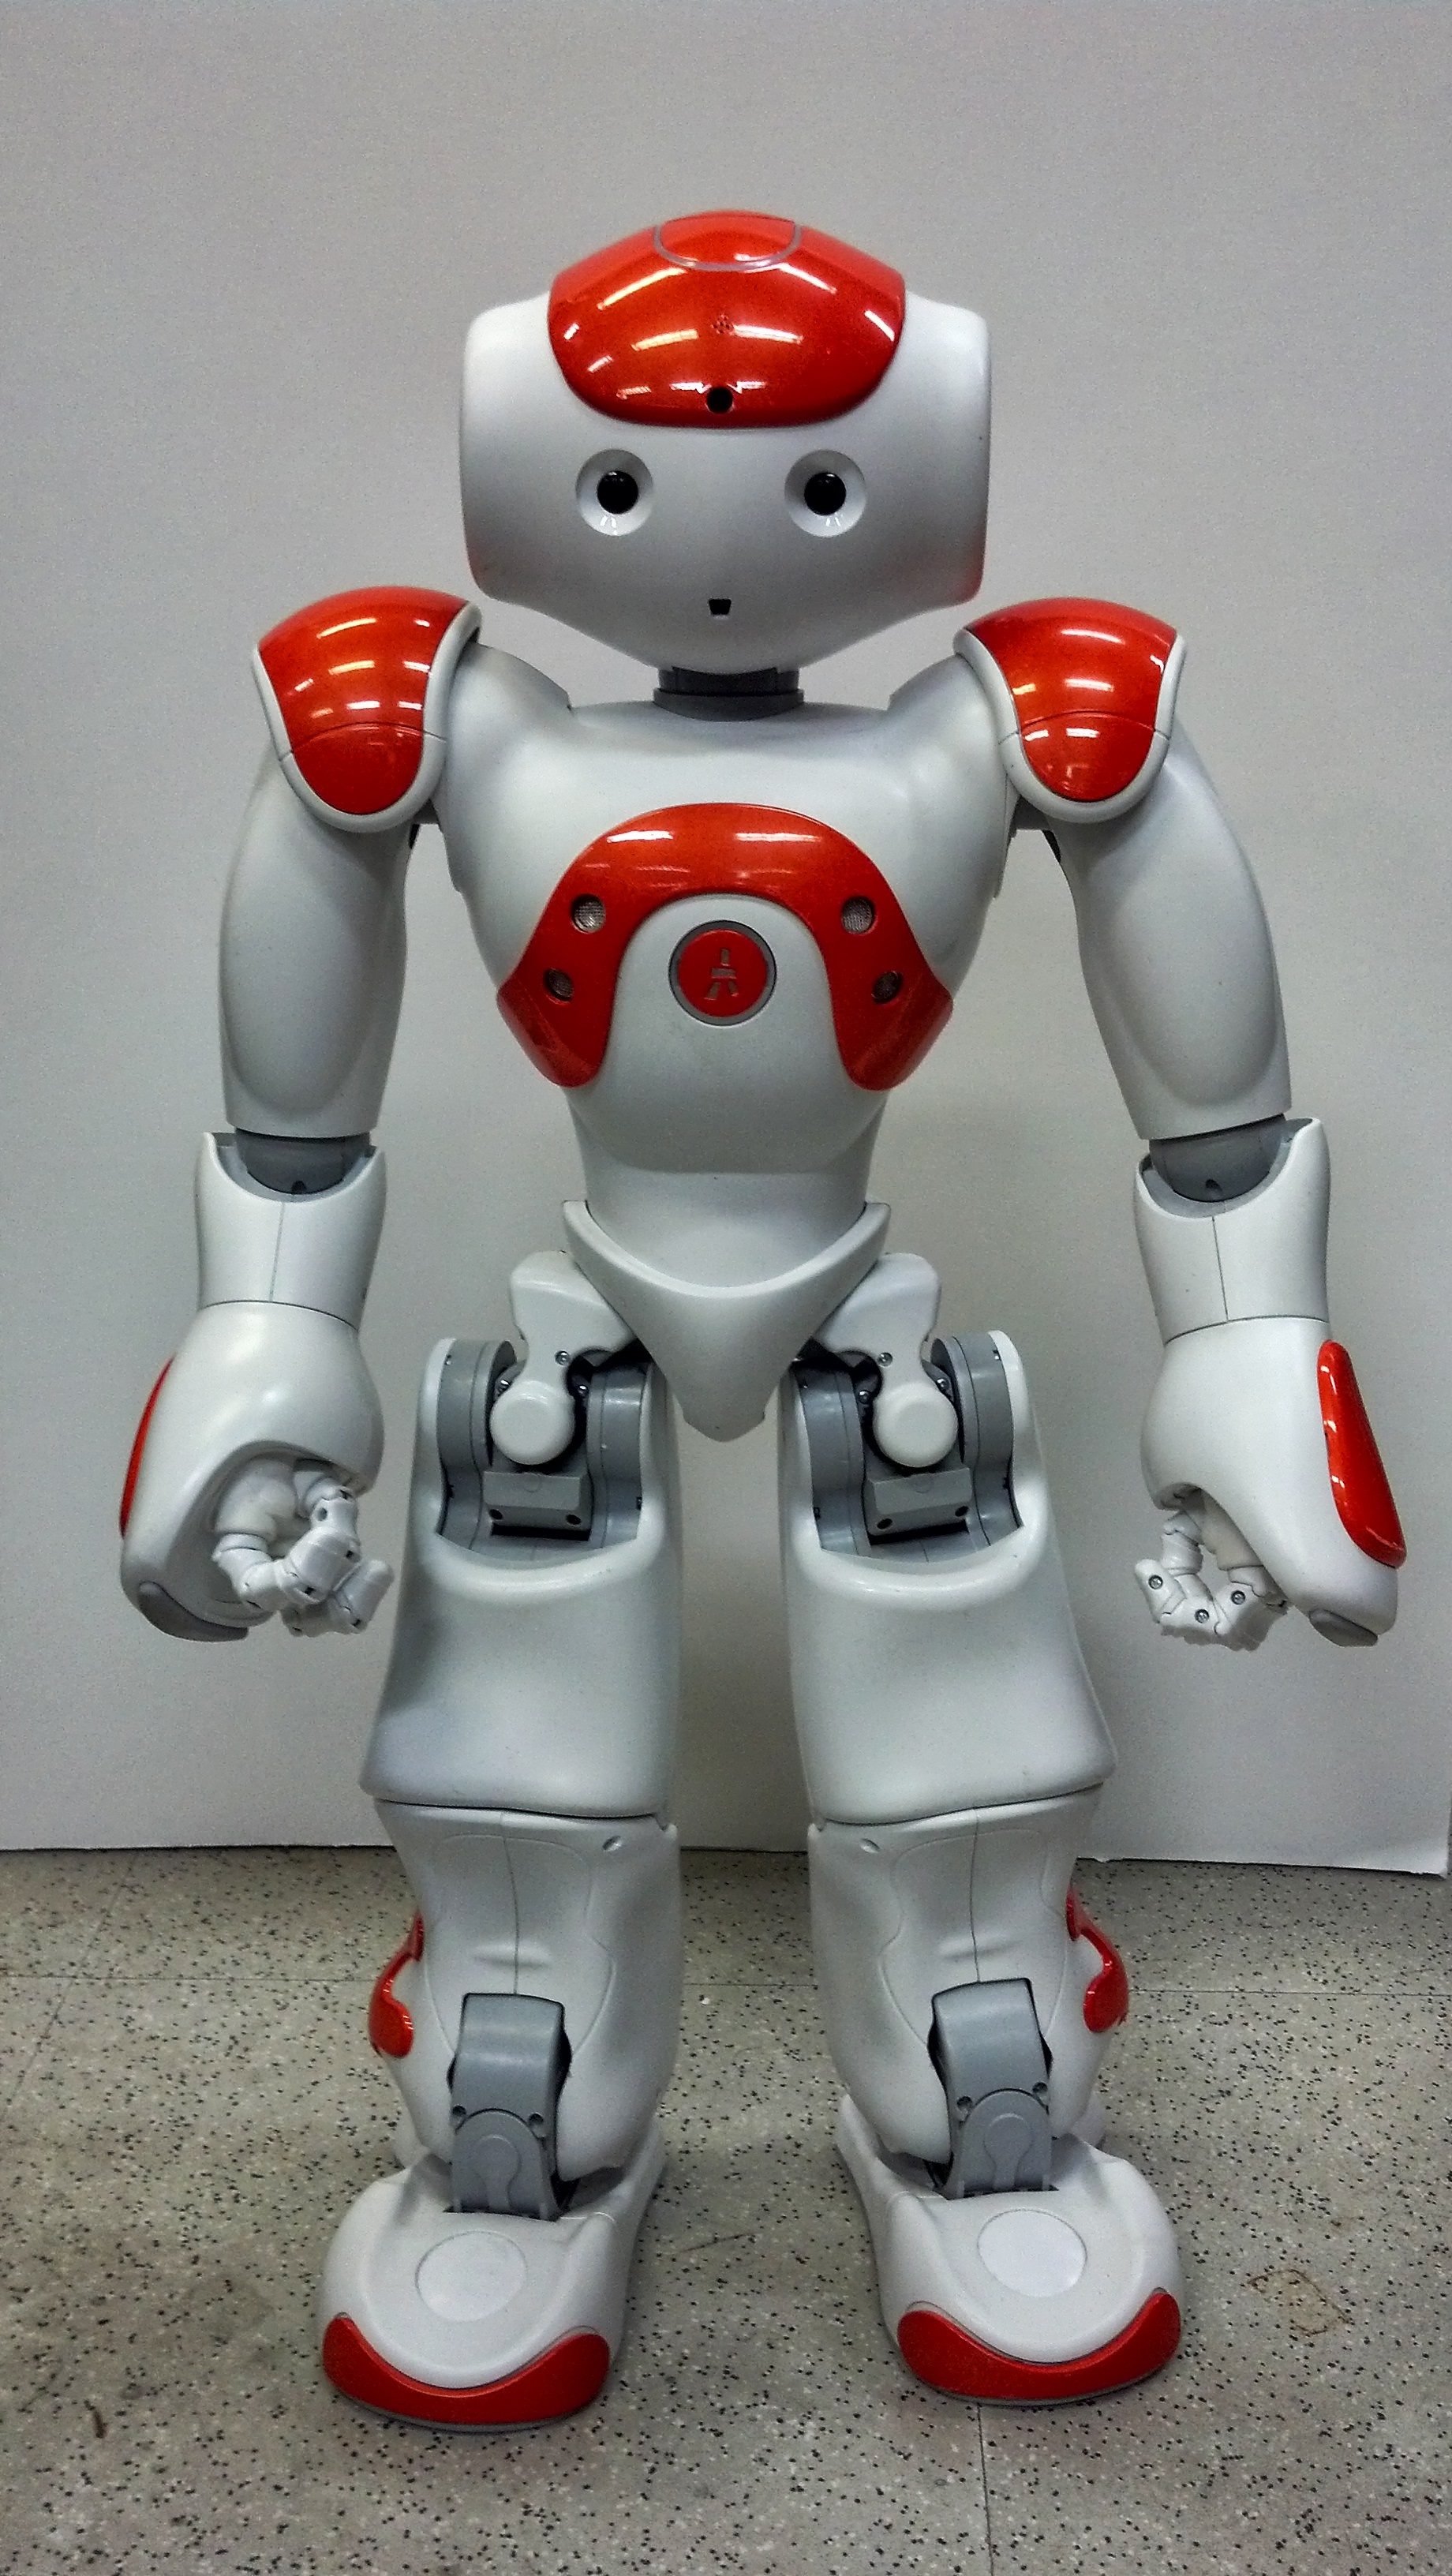
\includegraphics[width=0.35\textwidth]{nao1.jpg}
	\caption
	{Nao robot at Control/Robotics Research Lab}
	\label{fig:nao1}
\end{figure}

\section{Distance Sensors}\label{sec:sonar_section}
Two ultrasonic sensors in the chest allow for distance measurements to occlusions. Each sensor returns a single reading per measurement update as a distance reading in meters. This measurement is intended to represent the distance to the closest object within the sonar's field of view.
The transmitters are mounted at an angle of 20 degrees from the forward direction of the Nao and the receivers are mounted at 25 degrees. They have a 60 degree viewing angle with a detection range between 0.25 and 2.55 meters with a 1 cm resolution. 

\begin{figure}[h]
	\centering
	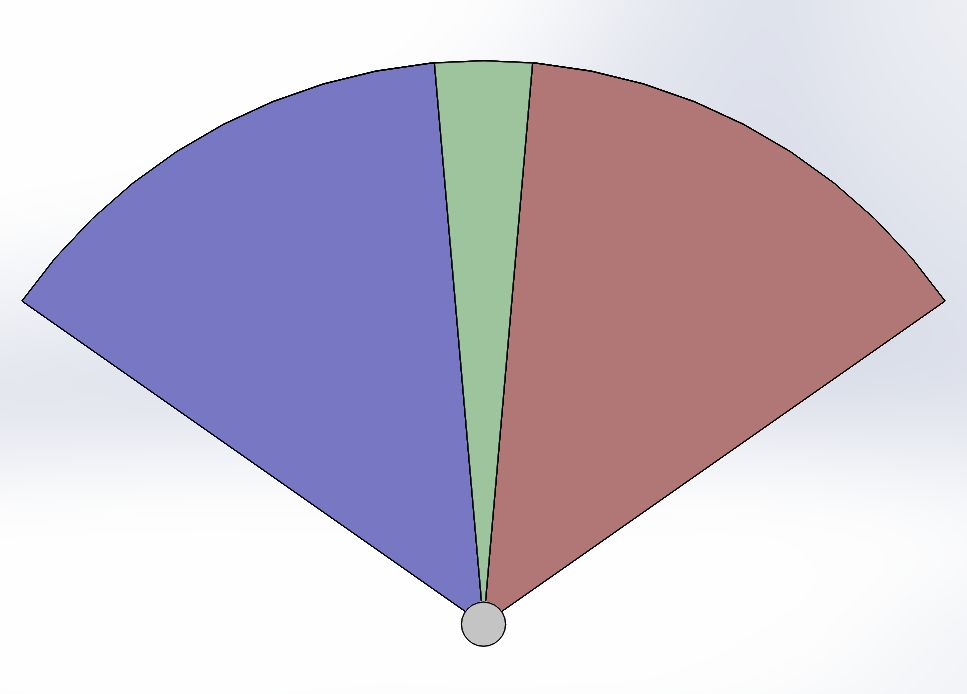
\includegraphics[width=0.35\textwidth]{sonar1.jpg}
	\caption
	[Nao sonar cones.]
	{Nao sonar cones. The left cone is shown in blue and the right cone is shown in red. The green cone shows the overlap between the two.}
	\label{fig:sonar1}
\end{figure}

As shown in Figure \ref{fig:sonar1}, the regions covered by the two ultrasonic sensors overlap. As the sensors do not report the angular position of the occlusion within the cone, uncertainty about the location of detected objects is high as they could be anywhere within the sonar cone.

The distance measurements also suffer from multipath returns and specular reflections which cause the robot to read incorrect distances at certain angles. For example, at times when the Nao is oriented toward a wall at an obtuse angle, the right distance sensor, which was closer to the wall, will read a distance much larger than that of the left sensor, causing the robot to gravitate into the wall. An example of the problem can be seen in Figure \ref{fig:sonar2}.

\begin{figure}[h]
	\centering
	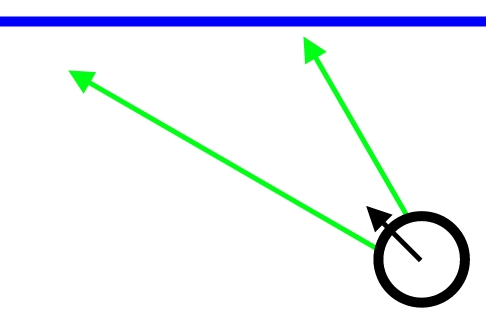
\includegraphics[width=0.35\textwidth]{sonar2.jpg}
	\caption
	[Distance measurement error at obtuse angles.]
	{Distance measurement error at obtuse angles. In the figure, the black circle represents the Nao in the plane, 
		while black arrow represents the current heading. The blue line represents a wall and the green arrows indicate
		the direction the sonars are pointing. When in positions similar to this the right sensor would report a distance
		greater than the left sensor, even though the right sensor is closer to the wall.}
	\label{fig:sonar2}
\end{figure}

At times, the source of erroneous sensor measurements stem from the material that the occlusion is made from. It was found that if the material is too soft, the distance reported to it will be larger, or at times, not be seen. Harder materials seem to correct for this. Soft materials are items like plastic trash cans. Metal trash cans respond more reliably.
A brief overview about various issues with sonar can be read about in \cite{sonar_issues1}.

\section{Programming}
There are three ways to program the Nao. The first is to use the graphical environment Choreographe. It is a block-based programming method where the user drags modules into an area and connects the modules together with arrows, to create a program flow. These modules can either be prebuilt or made by the programmer. The programmer can make their own modules by either dragging basic modules together and conglomerating them into a new module or they can program these modules using a text-based language, such as Python.
The second and third ways each involve using the framework provided by Aldebaran Robotics called NAOqi. NAOqi allows for many functions necessary for roboticists such as parallelism, resource management, and event synchronization while being cross-platform and cross-language\cite{NAOqi_overview1}. This API allows the programmer to take advantage of more of the resources available on Nao. NAOqi can be utilized in two ways. Either the projects built with NAOqi can be compiled for the linux distribution on Nao and then uploaded to it and executed, or the project can be compiled and run on an external computer and the commands sent to Nao over a network connection.
For this work, code is not compiled on the Nao itself but rather on an external computer and commands are sent to the Nao via a Wi-Fi network that both the Nao and the external computer are connected to. 
After setting up the build system qiBuild \cite{qiBuild_tutorial1} on the external computer, a new project is built using qiBuild and then edited and complied using Visual Studio 2008. Once built, the executable from the project is run from the command line with the IP address of the Nao as an argument and the Nao responds. Any print statements are seen on the command line.

The NAOqi framework uses the concept of proxies in order to access sensor data or send movement commands. Proxies are objects where data is accessed, stored, or sent. They are proxy to where these items are actually used or accessed, which are the Nao's memory, referenced using memory keys \cite{memory1}. For example, the memory keys for accessing the distance measurements for the sonar are:
\lstset{language=C++}
\begin{lstlisting}
	Device/SubDeviceList/US/Right/Sensor/Value
	Device/SubDeviceList/US/Left/Sensor/Value
\end{lstlisting}

More about the sonars can be read about in \cite{sonar_ref1}.

To initiate the updating of the sonars, the sonar proxy must be initialized with the IP address of the Nao and then subscribed to by the module. The module parameter is simply a keyword for your application. It is of your choosing. In this case the string \lstinline$"RAPlanner"$ was chosen. This will allow us to poll the distance readings rather than having to subscribe to events and provide callback functions.\cite{sonar_ref2}\cite{sonar_ref3}

\begin{lstlisting}
	AL::ALSonarProxy sonarPrx(argv[1], 9559);
	sonarPrx.subscribe("RAPlanner");
\end{lstlisting}
\lstinline$9559$ is the default port that NAOqi listens to. \lstinline$argv[1]$ contains the IP address of the Nao, as it is the first parameter in the command line argument when the executable is called.
To access the sensor data a memory proxy must be used as this data is stored in memory.

\begin{lstlisting}
	AL::ALMemoryProxy memPrxSonar(argv[1], 9559);
\end{lstlisting}
In the main loop, these values are accessed through methods of the proxy.

\begin{lstlisting}
	rightDist = memPrxSonar.getData(keyR);
	leftDist = memPrxSonar.getData(keyL);
\end{lstlisting}
where \lstinline$keyR$ and \lstinline$keyL$ are the const string key values of where the data is stored, \lstinline$"Device/SubDeviceList/US/Right/Sensor/Value"$ and \lstinline$"Device/SubDeviceList/US/Left/Sensor/Value"$ in this case. \lstinline$rightDist$ and \lstinline$leftDist$ are of type \lstinline$AL::ALValue$ which are later cast to floats for use by the path planning algorithm. The data is returned in meters.

To send motion commands to the Nao, a motion proxy must be used. The proxy must be initialized and the walk can be started.

\begin{lstlisting}
	AL::ALMotionProxy motionPrx(argv[1], 9559);
	motionPrx.walkInit();
\end{lstlisting}

As the Nao has not been given any movement commands, it will not move. Movements can be sent to it using a number of APIs \cite{naodoc_motion2}. The one used for this project was:

\begin{lstlisting}  
motionPrx.setWalkTargetVelocity(Vx, Vy, Om, stepFreq);
\end{lstlisting}

The method takes three different velocity commands, forward, lateral, and angular, in terms of fraction of maximum step length, and step frequency. \lstinline$Vx$, \lstinline$Vy$, \lstinline$Om$, \lstinline$stepFreq$ were floats passed into the method, updated by the path planning algorithm on every iteration of the main loop. The maximum step length is 8 cm forward, 16 cm laterally, and 0.523 radians angularly. The maximum step frequency is 2.381 Hz. Due to a stability controller in the built-in gaiting algorithm for the Nao, it takes 0.8 seconds for the robot to react to new commands. At maximum step frequency, this equates to about 2 steps \cite{naodoc_motion1}. The Nao can be stopped by setting all of the target velocities to zero.

For goal estimation, the inbuilt red ball tracker API is used. The red ball tracker returns the estimated position of a 6 cm red ball in 3-space, in the frame of the Nao's torso in meters \cite{naodoc_track1}.
In addition to the red ball tracker proxy being initialized and the tracker started, the Nao's head stiffness needs to be set. "Stiffness" refers to the percentage of available torque used in order to have a joint reach a target angle \cite{naodoc_stiff1}. The "Head" is a kinematic chain which refers to a collection of joints, in this case the yaw and pitch axes of the head \cite{naodoc_motion3}. A stiffness of 1.0 instructs the Nao to use all available torque to control the joint.

\begin{lstlisting}
	motionPrx.setStiffnesses("Head", 1.0f);
	AL::ALRedBallTrackerProxy redBallPrx(argv[1], 9559);
	redBallPrx.startTracker();
\end{lstlisting}

Following this, in the main loop new data is checked for and then accessed.
\begin{lstlisting}
	if(redBallPrx.isNewData()){}
		ballPose = redBallPrx.getPosition();
	}
\end{lstlisting}
\lstinline$getPosition()$ returns a vector of floats in x,y,z which was then passed to the path planning algorithm as the goal location.

A number of other program enhancements were made including initial head orienting and being able to push Nao's head buttons in order to set velocities to zero. All of these enhancements had a similar structure to the above code and can be read in Appendix \ref{chap:nao_code}



